\chapter{I teoremi di Rice e di Rice-Shapiro}

Andiamo ora a vedere un teorema importante: il teorema di Rice.

Pensiamo alla proprietà $P(i) = ``\forall n, \phii(n) \geq k$''. Possiamo già intuire dalla
quantificazione universale che la mia proprietà non è decidibile. Inoltre rimane il problema della
divergenza. Un'altra proprietà interessante è analoga ma ha il quantificatore esistenziale al
posto di quello universale. Questa è semidecidibile sicuramente, muovendosi con dove-tailing su input
e tempo. È decidibile? Intuitivamente no, dovrei fare una ricerca su uno spazio infinito. Se sono
fortunato in questi casi ho una proprietà semidecidibile.

Quello che andiamo a dimostrare adesso è che riguardo alle proprietà dei programmi non possiamo
decidere niente. Non esiste alcuna proprietà decidibile, ad esclusione delle proprietà di
falsità/verità costanti. Questo è dimostrabile in generale.

Questo qua è il succo del teorema di Rice.

\section{Proprietà estensionali}

Come caratterizziamo il comportamento delle funzioni calcolate dai programmi? Nel seguente modo:
data una proprietà $P$ ci chiediamo se $\phii = \phij$ implicihi $P(i) = P(j)$. Se questo è il
caso allora dico che $P$ è estensionale rispetto a $\phi$. È importante il legame con l'enumerazione,
che dato un numero mi restituisce la funzione calcolata dal programma con indice quel numero.

Possiamo caratterizzare un predicato con l'insieme degli indici delle funzioni per cui il predicato
è vero. Parliamo in generale di insiemi estensionali. $A$ è estensionale se $c_{A}$ è tale
che $\phii = \phij \implies c_{A}(i) = c_{A}(j)$. Gli insiemi estensionali sono chiusi rispetto a
complementazione, unione e intersezione; formano quindi un'algebra di Boole.

$\phi$ è una funzione dai naturali alle funzioni parziali calcolabili: $\phi : \Nat \to \PC$.
Prendiamo $B \subseteq \PC$. $A$ è estensionale se $A = \phi^{-1}(B)$. Queste due caratterizzazioni
sono equivalenti. La dimostrazione è lasciata al lettore.

\section{Il teorema di Rice}

\begin{thm}
    Un insieme $A$ estensionale è ricorsivo sse $A = \emptyset$ o $A = \Nat$ (o, equivalentemente,
    $A$ è banale).
\end{thm}

Banale in matematica significa solitamente degenere.

\begin{proof}
    L'implicazione inversa è banale. Dimostriamo solo quella diretta. Sia $A$ estensionale.
    Supponiamo che $A$ sia ricorsivo. Vogliamo dimostrare che $A$ è vuoto oppure $A = \Nat$.
    Procediamo per assurdo. Supponiamo che $A \not= \emptyset$ e $A \not= \Nat$. Esistono
    allora $a_{0} \in A$ e $a_{1} \notin A$. Sia $m$ un indice per la funzione che diverge sempre.
    Abbiamo due casi: o $m \in A$ o $m \in \comp{A}$. I due casi sono assolutamente simmetrici.
    Supponiamo, senza perdita di generalità, che $m \in \comp{A}$. A seconda che $\phii(i)$ converga
    o diverga voglio costruire un programma che ha lo stesso comportamento di $m$ in un caso e lo
    stesso comportamento di $a_{0}$ nell'altro. Vogliamo $g$ tale che:
    \begin{equation*}
        g(i,x) = 
        \begin{cases}
            \case{\phi_{a_{0}}(x)}{se $\phii(i) \converges$} \\
            \case{\phi_{m}(x)}{se $\phii(i) \diverges$} \\
        \end{cases}
    \end{equation*}
    Per s-m-n abbiamo $\phi_{s(i)}(x) = g(i,x)$. Come calcoliamo $g(i,x)$? Col seguente algoritmo:
    $g(i,x) = \phii(i); \phi_{a_{0}}(x)$. Di conseguenza $g$ è calcolabile. 
    
    Ci chiediamo ora: $s(i) \in A$? Dipende se $\phii(i)$ converge. $s(i) \in A \iff \phii(i)
    \converges$. Ma quindi anche $K$ sarebbe ricorsivo. Ma questo è assurdo.
\end{proof}

\section{Teorema di Rice-Shapiro}

\subsection{Proprietà compatte e monotone}

Cerchiamo ora di generalizzare il teorema di Rice. Cosa possiamo semidecidere del comportamento dei
programmi, tenuto vero quanto espresso dal teorema di Rice?

Prendiamo la proprietà essere totali: $P(i) = ``\phii \text{ è totale}$''. Intuitivamente questa proprietà non
è semidecidibile, perché dovrei esplorare tutti gli input prima di rispondere.

Proviamo con il complementare. Con un pò di abuso di notazione scriviamo $\comp{P}(i) = ``\phii
\text{ non è totale''} = ``\exists n, \phii(n) \diverges$''. La divergenza non è testabile: si tratta
sempre di una ricerca in uno spazio infinito, dove l'infinità è data dal tempo. Per questo motivo
neanche questa proprietà è semidecibile, almeno a livello intuitivo.

Cosa posso sicuramente semidecidere? La convergenza puntuale ad esempio. L'algoritmo è semplice:
lancio il programma $i$ sul mio input $x$ e aspetto. Se converge mi restituirà qualcosa, altrimenti
divergerà.

Intuitivamente, le proprietà semidecidibili sono i test che riguardano la convergenza su un numero
finito di input e i risultati relativi. Questo assomiglia un pò alla procedura di testing:
osserviamo il comportamento del programma su un numero finito di input e verifichiamo se passa il
mio test. È un testing semidecidibile. La cosa importante è che sia finito, non è neanche
richiesto che sia determinato.

Ad esempio, prendiamo $P(i) = ``\exists n, \phi_{i}(n) \converges$''. Questo test è chiaramente
semidecibie, mediante dove-tailing su $n$ e tempo.

Vogliamo ora formalizzare l'idea di cosa è semidecidibile e cosa no. Cerchiamo alcune proprietà
interessanti che sono soddisfatte da questi test.

Ci serve un ordinamento tra funzioni. Cerchiamo una nozione di ordinamento basata sul grafo delle
funzioni. Diciamo che $\phii \subseteq \phij$ se $\textit{grafo}(\phii) \subseteq
\textit{grafo}(\phij)$. In simboli questo corrisponde a $\forall n \forall m, \phii(n) = m \implies
\phij(n) = m$. Quand'è che $j$ può avere un comportamento diverso da $i$? Quando $i$ diverge. In
questo senso $j$ è una ``estensione'' di $i$.

$\phii \subseteq \phii$, in base alla nostra definizione. $\phij$ è, in un certo senso, più
informativa di $\phii$, dato che dove $\phii$ è definita il suo valore è identico a quello di
$\phij$, e dove $\phii$ non è definita $\phij$ può darmi una nuova informazione.

Qualunque funzione è un'estensione della funzione che diverge sempre. Sia $P(i)$ una proprietà
``testabile''. Supponiamo che $P(i)$ e supponiamo che $\phii \subseteq \phij$. Cosa possiamo dire su
$\phij$ rispetto a $P$? Per fissare le idee, prendiamo $P(i)$ = ``$\phii \text{ converge su tutti i
numeri minori di 100}$''. Supponiamo esista un $a$ per cui vale $P$. Se ho che $b$ estende $a$, ovvero
$\phia \subseteq \phib$, allora necessariamente $P(b)$: qualunque estensione di un programma che
converge su input minori di 100 continuerà a farlo.

Un predicato che rispetta la proprietà appena discussa è detto monotono. La monotonia è una
proprietà del mio predicato $P$ se per ogni estensione del mio programma $a$ per cui vale $P$
continua a valere la proprietà $P$. 

Vediamo ora un'altra caratteristica che può avere un predicato estensionale. Supponiamo di avere il
nostro test e che il test sia vero per un certo programma $a$. Allora, se esiste un $b$ tale $\phib$ è
una restrizione finita di $\phia$ e $P(b)$, diciamo che $P$ è compatto. Equivalentemente possiamo
esprimere la compattezza come $\exists b$ tale che $\phib \subseteq \phia$, $\phib$ è finito (come grafo)
e $P(b)$. Questa proprietà dei predicati estensionali è detta compattezza.

Abbiamo dei massimi nell'ordinamento basato su estensione? Sì, tutte le funzioni totali, dette in
questo contesto massimali. Non sono però in relazione tra loro, sono distinte.

\begin{figure}[!h]
    \centering
    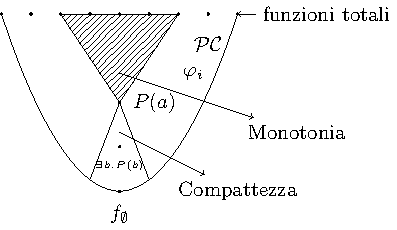
\includegraphics{img/ExtensionHierarchy.pdf}
    \caption{Una proprietà $P$ è monotona se tutte vale per tutte le estensioni di una funzione $a$
    per cui vale. È compatta se vale per una qualche restrizione finita $b$ di $a$}
\end{figure}

\newpage

Vediamo ora alcuni esempi di proprietà e chiediamoci quali sono compatte e quali monotone (e quali
entrambe).
\begin{itemize}
    \item $P(i) = ``\phii$ è totale''. È monotona? Sì. È compatta? No.
    \item $P(i) = ``\phii$ non è totale''. È monotona? No. È compatta? Sì.
    \item $P(i) = ``4 \in \cod(\phii)$''. È monotona? Sì. È compatta? Sì.
    \item $P(i) = ``\cod(\phii) = {4}$''. È monotona? No. È compatta? Sì.
\end{itemize}

Dimostreremo che monotonia e compattezza sono condizioni necessarie ma non sufficienti per la
semidecidibilità.

Prendiamo $P(i) = ``\dom(\phii)$ finito''. È monotona? No. È compatta? Sì. Per il complementare? È
monotono? Sì. È compatto? No.

%Prendiamo $P(i) = ``\dom(\phii)$ infinito e $\comp{\dom(\phii)}$ finito (?)''. È monotona? No. È
%compatta? No.

Una proprietà come $P(i) = `` \phii$ è primitiva ricorsiva'' non è neppure semidecidibile, oltre a non
essere decidibile per il teorema di Rice. Il motivo è che $P(i)$ non è compatta: il formalismo
primitivo ricorsivo mi permette di definire solo funzioni totali.

\subsection{Il teorema di Rice-Shapiro}

I nomi di questo teorema variano nella letteratura. Per noi è il teorema di Rice-Shapiro.

\begin{figure}[h]
    \centering
    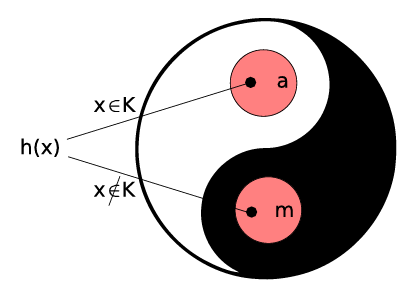
\includegraphics[scale=0.5]{img/YinYang.jpg}
    \caption{Visualizzazione della dimostrazione del teorema di Rice}
\end{figure}

\newpage

Il simbolo dello yin-yang mi deve sottolineare l'impossibilità di separare le due aree, perché le
due cose che sto tentando di separare sono processi in movimento che continuamente si trasformano
nell'una e nell'altra. Non posso operare una distinzione tra le due.

I due cerchi rappresentano degli intorni che non cambiano, che appartengono all'altra area. Da un
punto di vista topologico sono due aperti. Due aperti non possono dividere uno spazio, perché il
complementare di un aperto è un chiuso.

Possiamo immaginare un cerchio come un intorno di tutti i programmi che hanno lo stesso
comportamento di un certo programma. Se cerchiamo di dividere l'insieme di tutti i programmi in due
spazi non possiamo aspettarci di poterlo fare in modo algoritmico. Questo è il succo del teorema
di Rice. La proprietà di estensionalità, che è una proprietà di chiusura, non ci permette di
fare questa divisione.

Nella mia dimostrazione cerco un $s$ che mi permette di trovare una funzione che si comporta come
$a$ o $m$ a seconda del comportamento di $\phii(i)$. Questo lo posso fare, è più debole di
chiedere che $s(i)$ mi restituisca $a$ o $m$ a seconda del comportamento di $\phix(x)$ e sfrutta
l'estensionalità. La prima cosa posso calcolarla, la seconda no.

\begin{thm}
    \textbf{Teorema di Rice-Shapiro. }Sia $A$ un insieme estensionale. Se $A$ è r.e. allora:
    \begin{itemize}
        \item $A$ è monotono
        \item $A$ è compatto
    \end{itemize}
\end{thm}
\begin{proof}
    La monotonia mi dice che $\forall i,j$ se $i \in A$ e $\phii \subseteq \phij$ allora $j \in
    A$. Supponiamo che $A$ sia estensionale e r.e. Supponiamo che $A$ non sia monotono. Allora
    devono esistere $i,j$ tali che $i \in A$, $\phii \subseteq \phij$ e $j \notin A$. Proveremo a
    costruire un programma che si comporta come $i$ in un caso e come $j$ nell'altro caso.
    Costruiamo $h$ totale e calcolabile che vogliamo si comporti come $i$ se $\phix(x) \diverges$,
    come $j$ se $\phix(x) \converges$. Supponiamo di averla già: vedremo poi se possiamo
    calcolarla. Avremmo che $\phix(x) \in \comp{K} \iff h(x) \in A$. L'implicazione inversa di questo
    $\iff$ può essere dimostrata dimostrando $\lnot B \implies \lnot A$. Ma questo vuol dire che se
    $A$ fosse semidecidibile avrei un modo per calcolare, in modo semidecidibile, l'appartenenza a
    $\comp{K}$. 

    Tornando alla definizione del programma che calcola $h$, con s-m-n passiamo a $\phi_{h(x)} = g(x,y)
    = \phii(y) || (\phix(x)\phij(y))$. Questo programma ha lo stesso comportamento di $j$ anche se
    $\phix(x)$ converge e termina prima $\phii(y)$ perché $j$ è un'estensione di $i$. 

    Questa dimostrazione non è costruttiva. È costruttiva invece la dimostrazione per
    contraddizione: $A$ non monotono $\implies A$ non r.e.

    Questa dimostrazione implica, come corollario, il teorema di Rice.

    Passiamo alla compattezza. Questa mi dice che $\forall i, i \in A \implies \exists j, \phij \subseteq
    \phii, \phij$ è finita, $j \in A$.

    Andiamo nuovamente per assurdo. Andiamo a negare la compattezza di $A$: $\exists i, i \in A
    \forall j, \phij \subseteq \phii, \phij$ è finita $\implies j \notin A$.

    Vogliamo costruire una funzione parametrica in $x$ tale che si comporti come $i$ se $\phix(x)
    \diverges$ e come una qualsiasi restrizione finita di $i$ quando $\phix(x) \converges$. La
    conclusione della dimostrazione è identica a quella della monotonia, quindi concentriamoci su
    $h$. 

    Utilizzando s-m-n abbiamo $\phi_{h(x)} = g(x,y)$, con
    \begin{equation*}
        g(x,y) =
        \begin{cases}
            \case{\phii(y)}{se $T^{3}(x,x,y)$ = False}\\
            \case{\diverges}{se $T^{3}(x,x,y)$ = True}
        \end{cases}
    \end{equation*}

    Analizziamo il comportamento di questo programma. Ipotizziamo che $\phix(x)$ sia divergente.
    Siamo nel primo caso, quindi il comportamento del mio programma è identico a quello di $\phii$.
    Se $\phix(x)$ converge invece ad un certo punto $T$ mi restituirà True e da lì in poi la
    risposta rimarrà quella. A quel punto la mia funzione diverge. Questa corrisponde ad una
    restrizione finita di $i$: non so quanto lunga, so che esiste. Questa funzione è calcolabile,
    quindi $h$ è calcolabile, da cui l'asserto.
\end{proof}
